\documentclass[11pt,letterpaper]{article}
\usepackage[T1]{fontenc}
\usepackage{lmodern}
\usepackage[margin=1in]{geometry}
\usepackage{amsmath,amssymb,amsthm,mathtools}
\usepackage{enumitem}
\usepackage{microtype}
\usepackage{xcolor}
\usepackage{tikz}
\usepackage[colorlinks=true,linkcolor=blue,citecolor=blue,urlcolor=blue]{hyperref}
\usepackage{bookmark}
\pdftrailerid{}
\pdfsuppressptexinfo=15

\newtheorem{theorem}{Theorem}[section]
\newtheorem{proposition}[theorem]{Proposition}
\newtheorem{lemma}[theorem]{Lemma}
\newtheorem{corollary}[theorem]{Corollary}
\theoremstyle{definition}
\newtheorem{definition}[theorem]{Definition}
\theoremstyle{remark}
\newtheorem{remark}[theorem]{Remark}
\numberwithin{equation}{section}
\setlist{itemsep=3pt,topsep=5pt}
\hypersetup{pdftitle={Talagrand's discrete-convexity conjecture},
  pdfauthor={OpenAI},
  pdfsubject={A positive solution to Talagrand's Research Problem 13.3.2}}

\newcommand{\unverified}[1]{\par\smallskip\noindent\fbox{\parbox{0.95\linewidth}{\textbf{Unverified step.} #1}}\par\smallskip}
\newcommand{\step}[1]{\medskip\noindent\textbf{#1.}\ }

\title{Talagrand's discrete-convexity conjecture}
\author{Rewritten for readability from the OpenAI manuscript of the same title}
\date{September 23, 2026}

\AddToHook{cmd/thebibliography/after}{\addcontentsline{toc}{section}{\refname}}

\begin{document}
\maketitle
\begin{abstract}
We prove Talagrand's discrete-convexity conjecture.
There is a universal integer $k$ (namely $k=2^{75}$) such that, whenever an
arbitrary family has Bernoulli product measure at least $1-1/k$, the sets not
contained in a union of $k$ members admit a cover of total cost at most $1/2$
at the same density.
The argument is presented as a sequence of individually checkable steps.
\end{abstract}

\section{The result and how it is proved}
\label{sec:introduction}

\subsection{Setting and main theorem}

Throughout, $N\ge1$ is an integer, $[N]=\{1,\ldots,N\}$, and $2^{[N]}$ is the
set of all subsets of $[N]$. We identify a subset of $[N]$ with its indicator
vector in $\{0,1\}^N$. A \emph{family} is any subset of $2^{[N]}$.

\begin{itemize}
\item \textbf{Product measure.} For $p\in(0,1)$, $\mu_p$ is the probability
measure on $2^{[N]}$ under which each element of $[N]$ is present independently
with probability $p$; that is, $\mu_p(\{S\})=p^{|S|}(1-p)^{N-|S|}$.
\item \textbf{Exceptional sets.} For a family $\mathcal D$ and an integer
$k\ge1$,
\begin{equation}
\label{eq:exceptional-definition}
E_k(\mathcal D)
=\bigl\{S\subseteq[N]:
  S\nsubseteq D_1\cup\cdots\cup D_k
  \text{ for all }D_1,\ldots,D_k\in\mathcal D\bigr\}.
\end{equation}
The members $D_1,\ldots,D_k$ may repeat and need not be disjoint.
\item \textbf{Covers and cost.} A family $\mathcal G$ \emph{covers} a family
$\mathcal A$ if every $S\in\mathcal A$ contains some $I\in\mathcal G$. The
members of $\mathcal G$ are called \emph{generators}. For $\rho\in(0,1)$ the
\emph{cost} of $\mathcal G$ at density $\rho$ is
\[
c_\rho(\mathcal G)=\sum_{I\in\mathcal G}\rho^{|I|}.
\]
\item \textbf{Smallness.} $\mathcal A$ is \emph{$p$-small} if it has a cover
$\mathcal G$ with $c_p(\mathcal G)\le1/2$.
\end{itemize}

Since $\mu_p\{S:I\subseteq S\}=p^{|I|}$, a cover $\mathcal G$ of $\mathcal A$
gives $\mu_p(\mathcal A)\le\sum_{I\in\mathcal G}p^{|I|}=c_p(\mathcal G)$ by the
union bound. So ``$p$-small'' is a certified form of ``$\mu_p$-measure at most
$1/2$''. Two trivial facts are used later: a cover of $\mathcal A$ covers every
subfamily of $\mathcal A$, and the empty family is covered by
$\mathcal G=\varnothing$ at cost~$0$.

\begin{theorem}
\label{thm:main}
Set $k=2^{75}$. For every integer $N\ge1$, every $p\in(0,1)$, and every
family $\mathcal D\subseteq2^{[N]}$,
\[
\mu_p(\mathcal D)\ge1-\frac1k
\quad\Longrightarrow\quad
E_k(\mathcal D)\text{ is }p\text{-small}.
\]
\end{theorem}

The constant is independent of $N$, $p$, and $\mathcal D$. The family
$\mathcal D$ is arbitrary; no monotonicity is assumed. For orientation: if
$\mathcal D=\{D:|D|\le a\}$, then the unions of $k$ members of $\mathcal D$ are
exactly the sets of size at most $ka$, so $E_k(\mathcal D)=\{S:|S|>ka\}$.

\subsection{Proof at a glance}
\label{sec:glance}

The proof has three parts.

\paragraph{Part A: a covering lemma (Lemma~\ref{lem:covering},
Section~\ref{sec:covering}).}
This is purely combinatorial. Let $\mathcal H$ be a family of $r$-element sets
(``edges'') with $|\mathcal H|\rho^r\le2^{h+1}$. Then the sets that contain at
least $2^{12h}$ edges can be covered at $\rho$-cost at most $3\cdot2^{-h}$.
The cover is found by the probabilistic method and has three kinds of
generators: small sets lying in unusually many edges; unions of randomly
sampled pairs of the remaining edges; and unions of $2^{12h}$-tuples of edges
none of whose pairs was sampled. The third kind is cheap because such a tuple
must avoid $2^{24h}$ independent sampling events.

\paragraph{Part B: a cover at reduced density
(Proposition~\ref{prop:half-density}, Section~\ref{sec:weights}).}
If $\mu_q(\mathcal F)\ge1/2$, then $E_{32}(\mathcal F)$ is $(q/2^{70})$-small.
Compared with Theorem~\ref{thm:main}, the hypothesis is weaker and only $32$
unions are used, but the cost is measured at the smaller density $q/2^{70}$.
The proof attaches a weight $w(U)\ge0$ to every $U\subseteq[N]$ and has four
steps.
\begin{enumerate}[label=\textbf{B\arabic*.}]
\item (Parseval.) $\sum_{U}q^{|U|}w(U)\le1$.
\item (Signed identity on a $32\times N$ array.) Every $S\in E_{32}(\mathcal F)$
satisfies $\sum_{\varnothing\ne U\subseteq S}w(U)^{16}\ge2^{-32}$.
\item (Construction.) Sets $U$ with $w(U)\ge2^{-64|U|}$ are taken as generators;
by B1 they cost at most $2^{-6}$ at density $q/2^{70}$. The remaining sets are
sorted into bins $\mathcal H_{r,h}$ by size $r$ and dyadic weight
$w(U)\approx2^{-h}$, where necessarily $h\ge64r$. By B1 each bin satisfies the
hypothesis of Lemma~\ref{lem:covering}, which covers all sets containing at
least $2^{12h}$ members of the bin.
\item (Why it is a cover.) A set $S$ containing no generator has fewer than
$2^{12h}$ subsets in each bin, each contributing at most $2^{-16h}$ to the sum
in B2. The total is far below $2^{-32}$, so $S\notin E_{32}(\mathcal F)$. This
is where $32$ rows are needed: the exponent $16$ must beat the $12$ from
Lemma~\ref{lem:covering}.
\end{enumerate}

\paragraph{Part C: back to the original density
(Section~\ref{sec:density}).}
Let $L=2^{70}$, so $k=32L$. If $Lp<1$, we couple $L$ random sets
$R_1,\ldots,R_L$ so that each has law $\mu_p$ and their union has law
$\mu_{Lp}$. By the union bound all $R_j$ lie in $\mathcal D$ with probability
at least $31/32$, so the family $\mathcal F$ of $L$-fold unions of members of
$\mathcal D$ has $\mu_{Lp}(\mathcal F)\ge1/2$. Part B with $q=Lp$ shows that
$E_{32}(\mathcal F)=E_{32L}(\mathcal D)$ is $(q/L)$-small, and $q/L=p$. If
$Lp\ge1$, a second coupling shows $E_k(\mathcal D)=\varnothing$.

\begin{center}
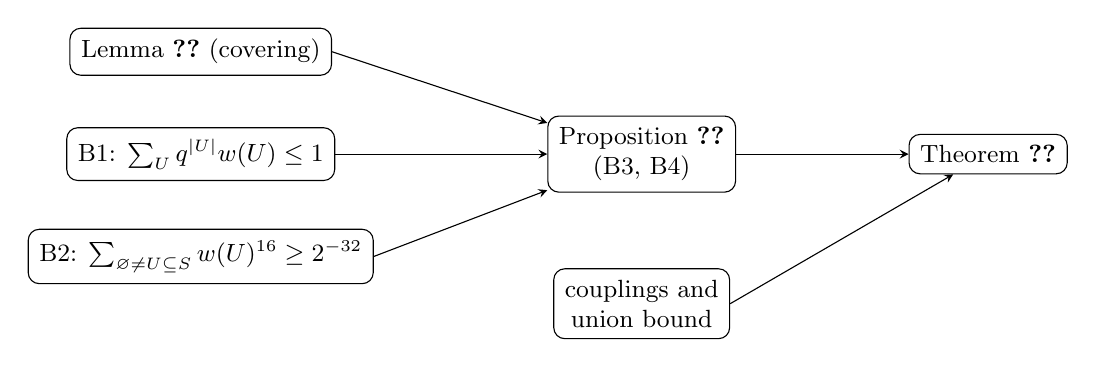
\begin{tikzpicture}[box/.style={draw,rounded corners,align=center,inner sep=4pt,font=\small},>=stealth]
\node[box] (lem) at (0,1.3) {Lemma~\ref{lem:covering} (covering)};
\node[box] (b1) at (0,0) {B1: $\sum_U q^{|U|}w(U)\le1$};
\node[box] (b2) at (0,-1.3) {B2: $\sum_{\varnothing\ne U\subseteq S}w(U)^{16}\ge2^{-32}$};
\node[box] (prop) at (5.6,0) {Proposition~\ref{prop:half-density}\\(B3, B4)};
\node[box] (cpl) at (5.6,-1.9) {couplings and\\union bound};
\node[box] (thm) at (10,0) {Theorem~\ref{thm:main}};
\draw[->] (lem.east) -- (prop);
\draw[->] (b1.east) -- (prop);
\draw[->] (b2.east) -- (prop);
\draw[->] (prop.east) -- (thm);
\draw[->] (cpl.east) -- (thm);
\end{tikzpicture}
\end{center}

Sections~\ref{sec:covering}, \ref{sec:weights} and \ref{sec:density} can be
read and checked independently, given the statements of
Lemma~\ref{lem:covering} and Proposition~\ref{prop:half-density}.
Section~\ref{sec:context} is context and is not used in the proof of
Theorem~\ref{thm:main}.

\paragraph{Renamed symbols.}
To keep one meaning per symbol we changed four names from the source. The
selector family $T$ is written $\mathcal T$ (Section~\ref{sec:context}). The
density $r=p/2$ in Corollary~\ref{cor:two-union} is written $p_0$. The tuple
length $t$ in Lemma~\ref{lem:covering} is written $\ell$. The signed column
mass $R$ in Proposition~\ref{prop:half-density} is written $\widetilde P$. We
also introduce the name $\kappa_U$ for a kernel that the source leaves
implicit.

\subsection{Context and consequences}
\label{sec:context}

\paragraph{Origin.}
The name reflects the analogy with Talagrand's Gaussian convexity
question~\cite[Conjecture~2.1]{Talagrand10}: can a bounded number of
sums of a compact balanced set of sufficiently large Gaussian measure
contain a convex set of Gaussian measure at least $1/2$, uniformly in
the dimension? (Balanced means closed under multiplication by scalars of
absolute value at most one.) In the discrete problem, unions replace sums and
containment covers describe the exceptional sets. Talagrand formulated the
discrete-convexity conjecture in \cite[Conjecture~7.1]{Talagrand10}; the same
original-density formulation appears as Research Problem~13.3.2
in~\cite{Talagrand21}, whose Proposition~13.3.3 explains its connection to
positive selector processes. Theorem~\ref{thm:main} proves this conjecture.

\paragraph{Positive selectors.}
The connection to positive selector processes \cite[Section~7]{Talagrand10}
gives a concrete consequence, recovering the positive-selector conclusion
proved by Park and Pham \cite[Theorem~1.2]{ParkPham24}. Let
$\mathcal T\subseteq[0,\infty)^N$ be nonempty and define
\[
\phi(S)=\sup_{\tau\in\mathcal T}\sum_{i\in S}\tau_i,
\qquad M=\mathbb E_{\mu_p}\phi,
\]
and suppose $0<M<\infty$. \emph{Claim: $\{S:\phi(S)\ge k^2M\}$ is $p$-small
for $k=2^{75}$.} The verification has three steps.
\begin{enumerate}[label=(\roman*)]
\item Put $\mathcal D=\{D:\phi(D)<kM\}$. Since $\phi\ge0$, Markov's inequality
gives $\mu_p\{\phi\ge kM\}\le M/(kM)=1/k$, so $\mu_p(\mathcal D)\ge1-1/k$.
\item $\phi$ is monotone and subadditive under unions. For $\tau\in\mathcal T$
all coordinates are nonnegative, so
$\sum_{i\in A\cup B}\tau_i\le\sum_{i\in A}\tau_i+\sum_{i\in B}\tau_i
\le\phi(A)+\phi(B)$, and $\sum_{i\in A}\tau_i\le\sum_{i\in B}\tau_i$ when
$A\subseteq B$. Take the supremum over $\tau$.
\item If $S\subseteq D_1\cup\cdots\cup D_k$ with all $D_j\in\mathcal D$, then by
(ii) $\phi(S)\le\sum_j\phi(D_j)<k\cdot kM$. Hence
$\{S:\phi(S)\ge k^2M\}\subseteq E_k(\mathcal D)$, and
Theorem~\ref{thm:main} supplies a cover of $E_k(\mathcal D)$ of $p$-cost at
most $1/2$.
\end{enumerate}
Thus the large-value event has explicit containment witnesses, beyond the
small probability already supplied by Markov's inequality.

\paragraph{Related developments.}
Hua, Song, and Tudose resolve Talagrand's Gaussian convexity problem and
derive a discrete conclusion with three unions and covering density
$p^C$, for a universal constant $C$, when the starting family is
sufficiently likely~\cite[Corollaries~1.3--1.4]{HuaSongTudose26}.
Ascoli, He, Park, and Talagrand give a threshold reformulation of discrete
convexity and prove cases for several graph-containment
properties~\cite[Proposition~1.5 and Theorems~1.10--1.13]{AscoliEtAl26}.

There is also a fractional version of smallness: instead of selecting
generators, one assigns nonnegative coefficients $a_I$ satisfying
\[
\sum_{I\subseteq S}a_I\ge1\quad(S\in\mathcal A),
\qquad
\sum_{I\subseteq[N]}p^{|I|}a_I\le\frac12.
\]
Talagrand introduced this relaxation alongside integral
smallness~\cite[Sections~6 and~7]{Talagrand10}.
Li resolves the fractional discrete-convexity problem through a quantitative
obstruction to probability measures whose containment probabilities
are bounded by $p^{|I|}$~\cite[Theorem~1.9]{Li26}.
Combining fractional information with rounding, Park obtains an integral
cover of $E_2(\mathcal D)$ at density
$p/\bigl(C\max\{1,\log\log(1/p)\}\bigr)$
whenever $\mu_p(\mathcal D)>1/2$, for a universal
$C$~\cite[Corollary~3.5]{Park26}.
Combining Li's result with the companion constant-factor rounding theorem
gives the following two-union tradeoff. Theorem~\ref{thm:main}, by contrast,
retains the original cost parameter $p$ while allowing a larger universal
number of unions.

\begin{corollary}[Two unions at constant density loss]
\label{cor:two-union}
There is a universal constant $C\ge1$ such that, for every integer $N\ge1$,
every $p\in(0,1)$, and every family $\mathcal D\subseteq2^{[N]}$,
\[
\mu_p(\mathcal D)>\frac12
\quad\Longrightarrow\quad
E_2(\mathcal D)\text{ is }(p/C)\text{-small}.
\]
\end{corollary}

\begin{proof}
The proof assembles three external results. Steps 1 and 3 are elementary.

\step{Step 1}
If $E_2(\mathcal D)=\varnothing$, the empty cover suffices. Otherwise
$\mathcal A=E_2(\mathcal D)$ is a nonempty proper increasing family. It is
proper because $\mathcal D\ne\varnothing$, so $\varnothing\subseteq D\cup D$
for some $D\in\mathcal D$ and $\varnothing\notin\mathcal A$. It is increasing
because $S\subseteq S'\subseteq D_1\cup D_2$ implies $S\subseteq D_1\cup D_2$.

\step{Step 2 (external)}
By Li's result \cite[Corollary~3.1]{Li26} in Park's fractional-cover
formulation \cite[Theorem~3.4]{Park26}, $\mathcal A$ has a fractional cover of
cost at most $1/2$ at density $p_0=p/2$: coefficients $a_I\ge0$ with
$\sum_{I\subseteq S}a_I\ge1$ for $S\in\mathcal A$ and
$\sum_Ip_0^{|I|}a_I\le1/2$.

\step{Step 3}
Replace each $a_I$ by $\min\{a_I,1\}$. The cost does not increase. Coverage is
preserved: if some $I\subseteq S$ had $a_I>1$, that term alone now equals $1$;
otherwise no term of $\sum_{I\subseteq S}a_I$ changed.

\step{Step 4 (external)}
The companion expectation-threshold
theorem~\cite[Theorem~1.1]{OpenAIThreshold26} then gives an integral cover of
cost at most $1/2$ at density $p_0/(25\cdot512^4)=p/(50\cdot512^4)$. Thus
$C=50\cdot512^4$ suffices.
\unverified{Steps 2 and 4 quote \cite{Li26}, \cite{Park26} and
\cite{OpenAIThreshold26} exactly as the source uses them. We did not have the
precise statements of these results, so we could not check their hypotheses
against Step~1 and Step~3, nor the constants $p/2$ and $25\cdot512^4$. The
corollary is not used in the proof of Theorem~\ref{thm:main}.}
\end{proof}

\paragraph{Antecedents of the method.}
The two-row version of the signed product in Section~\ref{sec:weights} is
Li's signed kernel after multiplication by the Bernoulli
masses~\cite[Section~2]{Li26}. The method has antecedents in the signed product
operators and biased Fourier analysis of
Friedgut~\cite[Section~2.2]{Friedgut08} and Ellis, Filmus, and
Friedgut~\cite[Sections~2.2 and~4.1]{EllisFilmusFriedgut12}. Random unions
also enter the covering constructions of Fischer and
Person~\cite[Sections~1.1 and~2]{FischerPerson25}; the covering lemma here is
proved in full.

\section{An elementary covering lemma}
\label{sec:covering}

This section is self-contained. Its lemma is used once, in Step~3 of the proof
of Proposition~\ref{prop:half-density}, where it is applied to each bin
$\mathcal H_{r,h}$. Covers and the cost $c_\rho$ are defined as in
Section~\ref{sec:introduction}, with a finite set $X$ in place of $[N]$;
$\binom Xr$ denotes the family of $r$-element subsets of $X$.

\begin{lemma}\label{lem:covering}
Let \(X\) be a finite set, let \(0<\rho<1\), and let \(r,h\) be integers
with \(1\le r\le h\) and \(h\ge64\). Suppose that
\(\mathcal H\subseteq\binom{X}{r}\) satisfies
\[
|\mathcal H|\rho^r\le2^{h+1}.
\]
Then the family
\[
\left\{S\subseteq X:
  |\{e\in\mathcal H:e\subseteq S\}|\ge2^{12h}\right\}
\]
has a cover \(\mathcal G\subseteq2^X\) with
\[
c_\rho(\mathcal G)\le3\cdot2^{-h}.
\]
\end{lemma}

\paragraph{Plan.}
Members of $\mathcal H$ are called \emph{edges}; the sets $S$ in the displayed
family are \emph{target sets}. We build
$\mathcal G=\mathcal C_0\cup\mathcal C_1\cup\mathcal C_2$, where
$\mathcal C_0$ is deterministic and $\mathcal C_1,\mathcal C_2$ depend on a
random sample of pairs of edges. We show that $\mathcal G$ is a cover for
\emph{every} outcome of the sample (Step~5) and that
$\mathbb E[c_\rho(\mathcal G)]\le3\cdot2^{-h}$ (Steps 1, 3, 6--9). Some
outcome then has cost at most the expectation.

\begin{proof}
\step{Step 0 (parameters)}
Put
\[
m=2^{12h},\qquad T=2^{4h},\qquad \pi=2^{-8h}.
\]
For \(I\subseteq X\) with \(|I|\le r\), define its \emph{weighted degree}
\[
d(I)=|\{e\in\mathcal H:I\subseteq e\}|\,\rho^{r-|I|}.
\]

\step{Step 1 (generators of large weighted degree)}
Let
\[
\mathcal C_0=\{I\subseteq X:|I|\le r,\ d(I)>T\}.
\]
\emph{Claim:} $c_\rho(\mathcal C_0)\le2^{1-2h}$.
Since $d(I)\rho^{|I|}=|\{e\in\mathcal H:I\subseteq e\}|\rho^r$, exchanging the
order of summation and using that an edge has exactly $2^r$ subsets gives
\begin{equation}\label{eq:cov-double}
\sum_{\substack{I\subseteq X\\|I|\le r}}d(I)\rho^{|I|}
=\sum_{e\in\mathcal H}\ \sum_{I\subseteq e}\rho^r
=2^r|\mathcal H|\rho^r.
\end{equation}
Each $I\in\mathcal C_0$ satisfies $1<d(I)/T$. Hence, by \eqref{eq:cov-double},
the hypothesis $|\mathcal H|\rho^r\le2^{h+1}$, and $r\le h$,
\begin{equation}\label{eq:cov-C0}
c_\rho(\mathcal C_0)
=\sum_{I\in\mathcal C_0}\rho^{|I|}
\le T^{-1}\sum_{I\in\mathcal C_0}d(I)\rho^{|I|}
\le T^{-1}2^r|\mathcal H|\rho^r
\le2^{-4h}\,2^r\,2^{h+1}
=2^{r+1-3h}\le2^{1-2h}.
\end{equation}

\step{Step 2 (regular edges and the extension bound)}
Call an edge \emph{regular} if it contains no member of \(\mathcal C_0\),
and let \(\mathcal H'\subseteq\mathcal H\) be the family of regular edges.
Every subset of an edge has size at most $r$, so by definition of
$\mathcal C_0$
\begin{equation}\label{eq:cov-regular}
I\subseteq e\in\mathcal H'
\quad\Longrightarrow\quad d(I)\le T.
\end{equation}
\emph{Claim (extension bound):} for every \(B\subseteq X\),
\begin{equation}\label{eq:cov-ext}
\sum_{e\in\mathcal H'}\rho^{|e\setminus B|}
\le T\sum_{i=0}^r\binom{|B|}{i}.
\end{equation}
To prove it, group the regular edges $e$ by their trace $I=e\cap B$. A trace is
a subset of $B$ of size at most $r$, so at most $\sum_{i=0}^r\binom{|B|}{i}$
traces occur. Fix a trace $I$ that occurs, say $I=e_0\cap B$ with
$e_0\in\mathcal H'$. Every edge $e$ with trace $I$ contains $I$ and has
$|e\setminus B|=r-|I|$, so
\[
\sum_{\substack{e\in\mathcal H'\\e\cap B=I}}
  \rho^{|e\setminus B|}
=|\{e\in\mathcal H':e\cap B=I\}|\,\rho^{r-|I|}
\le|\{e\in\mathcal H:I\subseteq e\}|\,\rho^{r-|I|}
=d(I)\le T,
\]
where the last inequality is \eqref{eq:cov-regular} applied to
$I\subseteq e_0$. Summing over the traces that occur gives \eqref{eq:cov-ext}.

\step{Step 3 (sampled pairs)}
Independently for each ordered pair \((e,e')\in(\mathcal H')^2\), including the
diagonal pairs $(e,e)$, \emph{sample} that pair with probability \(\pi\). Let
\(\mathcal C_1\) be the family of unions $e\cup e'$ of sampled pairs.
\emph{Claim:} $\mathbb E[c_\rho(\mathcal C_1)]\le2^{1-2h}$.
Apply \eqref{eq:cov-ext} with \(B=e\), so that $|B|=r$ and
$\sum_{i=0}^r\binom ri=2^r$:
\[
\sum_{e'\in\mathcal H'}\rho^{|e'\setminus e|}\le2^rT
\qquad(e\in\mathcal H').
\]
Each member of $\mathcal C_1$ is the union of at least one sampled pair, so
$c_\rho(\mathcal C_1)\le\sum_{(e,e')\text{ sampled}}\rho^{|e\cup e'|}$. Taking
expectations and using $\rho^{|e\cup e'|}=\rho^r\rho^{|e'\setminus e|}$,
\begin{align}
\mathbb E[c_\rho(\mathcal C_1)]
&\le\pi\sum_{e\in\mathcal H'}\rho^r\sum_{e'\in\mathcal H'}\rho^{|e'\setminus e|}
\le\pi\,|\mathcal H'|\rho^r\,2^rT
\notag\\
&\le2^{-8h}\,2^{h+1}\,2^r\,2^{4h}
=2^{r+1-3h}\le2^{1-2h}.
\label{eq:cov-C1}
\end{align}
Distinct ordered pairs are independent sampling indices even when their
unions coincide; the bound counts unions with multiplicity.

\step{Step 4 (residual generators)}
For every ordered tuple \((e_1,\ldots,e_m)\) of \emph{pairwise distinct}
regular edges, add \(e_1\cup\cdots\cup e_m\) to \(\mathcal C_2\) if none of the
pairs \((e_i,e_j)\), \(1\le i,j\le m\), was sampled. Put
\[
\mathcal G=\mathcal C_0\cup\mathcal C_1\cup\mathcal C_2.
\]
\unverified{The source defines $\mathcal C_2$ from ``every ordered tuple
$(e_1,\ldots,e_m)$ of regular edges'' and later asserts that the $m^2$ pair
indices of such a tuple ``are all distinct''. Read literally (repetitions
allowed) that assertion is false: the tuple $(e,\ldots,e)$ has the single
index $(e,e)$ and survives with probability $1-\pi$, so $\mathcal C_2$ would
cost about $|\mathcal H'|\rho^r$, which is only bounded by $2^{h+1}$. The
assertion is true for pairwise distinct edges, which is all Step~5 uses and
what the source's phrases ``$m$ distinct regular edges'' and ``not necessarily
distinct'' (for $W_\ell$) indicate. We adopt that reading; with it, every step
below checks.}

\step{Step 5 ($\mathcal G$ is a cover for every sampling outcome)}
Let $S$ be a target set. If $S$ contains a member of $\mathcal C_0$ we are
done. Otherwise every edge $e\subseteq S$ is regular, because a member of
$\mathcal C_0$ inside $e$ would lie inside $S$. So $S$ contains at least $m$
distinct regular edges; choose $m$ of them, $e_1,\ldots,e_m$. If some pair
$(e_i,e_j)$ was sampled, then $e_i\cup e_j\in\mathcal C_1$ and
$e_i\cup e_j\subseteq S$. If no such pair was sampled, then
$e_1\cup\cdots\cup e_m\in\mathcal C_2$ by Step~4, and it is contained in $S$.

\step{Step 6 (total weight of tuples)}
For \(0\le \ell\le m\), let
\[
W_\ell=
\sum_{(e_1,\ldots,e_\ell)\in(\mathcal H')^\ell}
  \rho^{|e_1\cup\cdots\cup e_\ell|},
\qquad W_0=1,
\]
where the edges in a tuple are \emph{not} required to be distinct.
\emph{Claim:}
\begin{equation}\label{eq:cov-W}
W_m\le\bigl[T(1+rm)^r\bigr]^m.
\end{equation}
Fix $\ell<m$ and a tuple $(e_1,\ldots,e_\ell)$ with union $B$; then
$|B|\le r\ell\le rm$. For any integer $n\ge0$ we have
$\sum_{i=0}^r\binom ni\le(1+n)^r$: order an $n$-set, and send each subset
$\{a_1<\cdots<a_i\}$ with $i\le r$ to the word
$(a_1,\ldots,a_i,\ast,\ldots,\ast)$ of length $r$ over the $n+1$ symbols
consisting of the $n$ elements and a new symbol $\ast$; this map is injective.
Since $\rho^{|B\cup e|}=\rho^{|B|}\rho^{|e\setminus B|}$,
\eqref{eq:cov-ext} gives
\[
\sum_{e\in\mathcal H'}\rho^{|B\cup e|}
\le\rho^{|B|}\,T(1+|B|)^r
\le\rho^{|B|}\,T(1+rm)^r.
\]
Summing over all tuples of length $\ell$ gives
$W_{\ell+1}\le T(1+rm)^rW_\ell$, and iterating from $W_0=1$ gives
\eqref{eq:cov-W}.

\step{Step 7 (expected cost of $\mathcal C_2$)}
Let $(e_1,\ldots,e_m)$ be a tuple of pairwise distinct regular edges. Then
$(i,j)\mapsto(e_i,e_j)$ is injective, so the tuple has exactly $m^2$ distinct
pair indices. They are sampled independently, so the probability that none is
sampled is
\[
(1-\pi)^{m^2}\le e^{-\pi m^2}\le2^{-\pi m^2}.
\]
Each member of $\mathcal C_2$ arises from at least one such surviving tuple,
and the sum of $\rho^{|e_1\cup\cdots\cup e_m|}$ over tuples of distinct edges
is at most $W_m$. By linearity of expectation and \eqref{eq:cov-W},
\[
\mathbb E[c_\rho(\mathcal C_2)]
\le W_m\,2^{-\pi m^2}
\le\bigl[T(1+rm)^r\bigr]^m\,2^{-\pi m^2}.
\]

\step{Step 8 (arithmetic)}
\emph{Claim:} $\mathbb E[c_\rho(\mathcal C_2)]\le2^{-m}$.
Using $r\le h$ and $h+1\le2^h$,
\[
1+rm\le(h+1)2^{12h}\le2^{13h},
\qquad\text{so}\qquad
T(1+rm)^r\le2^{4h+13rh}.
\]
Next, $\pi m=2^{-8h}2^{12h}=2^{4h}$, and
\begin{equation}\label{eq:cov-arith}
4h+13rh+1\le4h+13h^2+1\le18h^2
\le18\cdot2^{2h}\le2^{4h}=\pi m,
\end{equation}
using $r\le h$, then $4h+1\le5h^2$, then $h\le2^h$, then $18\le2^{2h}$ (true
for $h\ge3$). Therefore
\begin{equation}\label{eq:cov-C2}
\mathbb E[c_\rho(\mathcal C_2)]
\le2^{(4h+13rh)m-\pi m^2}
=2^{m(4h+13rh-\pi m)}\le2^{-m}.
\end{equation}

\step{Step 9 (conclusion)}
Cost is subadditive over unions of families, so by \eqref{eq:cov-C0},
\eqref{eq:cov-C1} and \eqref{eq:cov-C2},
\[
\mathbb E[c_\rho(\mathcal G)]
\le2^{1-2h}+2^{1-2h}+2^{-m}
=2^{2-2h}+2^{-m}\le2^{-h}+2^{-h}\le3\cdot2^{-h},
\]
where $2^{2-2h}\le2^{-h}$ because $h\ge2$, and $2^{-m}\le2^{-h}$ because
$m=2^{12h}\ge h$. All families and sampling indices are finite, so some
outcome has $c_\rho(\mathcal G)$ at most its expectation. By Step~5 that
outcome supplies a cover.
\end{proof}

\begin{remark}
The hypothesis $r\le h$ is used in \eqref{eq:cov-C0}, \eqref{eq:cov-C1} and
\eqref{eq:cov-arith}. Of the hypothesis $h\ge64$, the proof uses only $h\ge3$.
The lemma is applied with $h\ge64r\ge64$.
\end{remark}

\section{Weights for exceptional sets}
\label{sec:weights}

The following proposition is the theorem at a reduced density. It is used in
Case~1 of the proof of Theorem~\ref{thm:main}, with $q=Lp$.

\begin{proposition}\label{prop:half-density}
Let $L=2^{70}$. For every integer $N\ge1$, every $q\in(0,1)$, and every
$\mathcal F\subseteq 2^{[N]}$ satisfying $\mu_q(\mathcal F)\ge1/2$,
the family $E_{32}(\mathcal F)$ is $(q/L)$-small.
\end{proposition}

\paragraph{Plan.}
We define weights $w(U)\ge0$. Step~1 bounds $\sum_Uq^{|U|}w(U)$ by Parseval's
identity. Step~2 shows $\sum_{\varnothing\ne U\subseteq S}w(U)^{16}\ge2^{-32}$
for every exceptional $S$. Step~3 builds a cover from the heavy sets and from
Lemma~\ref{lem:covering} applied to dyadic bins, and bounds its cost by
Step~1. Step~4 shows by Step~2 that it covers $E_{32}(\mathcal F)$.

\begin{proof}
\step{Notation}
Write $f=\mathbf 1_{\mathcal F}:\{0,1\}^N\to\{0,1\}$ and
$\mu_q(x)=\prod_{i\in[N]}q^{x_i}(1-q)^{1-x_i}$. For $U\subseteq[N]$ and
$x\in\{0,1\}^N$ let
\begin{equation}\label{eq:kernel}
\kappa_U(x)=(1-q)^{|U|}\,(-1)^{\sum_{i\in U}x_i}
\prod_{i\in[N]\setminus U}q^{x_i}(1-q)^{1-x_i},
\end{equation}
and define
\begin{equation}\label{eq:b-def}
b(U)=\sum_{x\in\{0,1\}^N}\kappa_U(x)f(x),
\qquad w(U)=b(U)^2.
\end{equation}
Splitting $x$ into its restriction $z$ to $U$ and its restriction to
$[N]\setminus U$, this is the source's formula
\[
 b(U)=(1-q)^{|U|}
 \sum_{z\in\{0,1\}^{U}}(-1)^{\sum_{i\in U}z_i}\,
 \mathbb E[f(z,Y)],
\]
where $Y$ has independent Bernoulli-$q$ coordinates on $[N]\setminus U$ and
$(z,Y)$ is the point equal to $z$ on $U$ and to $Y$ elsewhere. Since
$\kappa_\varnothing=\mu_q$,
\[
b(\varnothing)=\mu_q(\mathcal F)\ge\tfrac12.
\]

\emph{Sanity check.} Take $N=1$, $q\le1/2$, $\mathcal F=\{\varnothing\}$. Then
$b(\varnothing)=1-q$ and $b(\{1\})=(1-q)\bigl(f(0)-f(1)\bigr)=1-q$. Here
$E_{32}(\mathcal F)=\{\{1\}\}$, and for $S=\{1\}$ the identity
\eqref{eq:signed-identity} below reads $(1-q)^{32}-(1-q)^{32}=0$.

\step{Step 1 (global weight bound)}
\emph{Claim:}
\begin{equation}\label{eq:global}
\sum_{U\subseteq[N]}q^{|U|}w(U)\le\mu_q(\mathcal F)\le1.
\end{equation}
We use the standard biased Fourier basis \cite[Section~8.4]{ODonnell14}, with
its normalization made explicit.

\emph{(a) Orthonormal basis.} For $U\subseteq[N]$ let
\[
 \chi_U(x)=\frac{\prod_{i\in U}(q-x_i)}{[q(1-q)]^{|U|/2}}.
\]
Under $X\sim\mu_q$ the coordinates are independent with
$\mathbb E[q-X_i]=0$ and $\mathbb E[(q-X_i)^2]=q(1-q)$. Hence
$\mathbb E[\chi_U\chi_V]$ is a product of factors $1$ over $i\in U\cap V$ and
factors $0$ over $i$ in the symmetric difference, so it equals $1$ if $U=V$
and $0$ otherwise. Since $0<q<1$, $\mu_q$ has full support, so
$\langle g,g'\rangle=\mathbb E[g(X)g'(X)]$ is an inner product on the
$2^N$-dimensional space of real functions on $\{0,1\}^N$, and the $2^N$
orthonormal functions $\chi_U$ form a basis. With
$\widehat f(U)=\mathbb E[f(X)\chi_U(X)]$, Parseval's identity reads
$\sum_U\widehat f(U)^2=\mathbb E[f(X)^2]$.

\emph{(b) Relation to $b$.} For $x_i\in\{0,1\}$,
\[
q^{x_i}(1-q)^{1-x_i}\,(q-x_i)=q(1-q)(-1)^{x_i},
\]
since the left side is $(1-q)q$ for $x_i=0$ and $q(q-1)$ for $x_i=1$. Applying
this to each $i\in U$,
\[
\mu_q(x)\chi_U(x)
=[q(1-q)]^{|U|/2}(-1)^{\sum_{i\in U}x_i}
\prod_{i\notin U}q^{x_i}(1-q)^{1-x_i}
=\Bigl(\frac{q}{1-q}\Bigr)^{|U|/2}\kappa_U(x).
\]
Multiplying by $f(x)$ and summing over $x$,
\[
\widehat f(U)=\Bigl(\frac{q}{1-q}\Bigr)^{|U|/2}b(U),
\qquad\text{hence}\qquad
q^{|U|}w(U)=(1-q)^{|U|}\widehat f(U)^2.
\]

\emph{(c) Conclusion.} Since $(1-q)^{|U|}\le1$ and $f^2=f$,
\[
 \sum_{U\subseteq[N]}q^{|U|}w(U)
 =\sum_{U\subseteq[N]}(1-q)^{|U|}\widehat f(U)^2
 \le\sum_{U\subseteq[N]}\widehat f(U)^2
 =\mathbb E[f(X)^2]
 =\mu_q(\mathcal F)\le1.
\]

\step{Step 2 (lower bound on every exceptional set)}
Fix $S\in E_{32}(\mathcal F)$. \emph{Claim:}
\begin{equation}\label{eq:exceptional}
 \sum_{\varnothing\ne U\subseteq S}w(U)^{16}\ge2^{-32}.
\end{equation}

\emph{(a) A signed weight on arrays.} Consider arrays
$\mathbf x=(x_{ji})\in\{0,1\}^{32\times N}$. Row $j$ is
$x_j=(x_{j1},\ldots,x_{jN})\in\{0,1\}^N$, a subset of $[N]$; column $i$ is
$x_{\bullet i}=(x_{1i},\ldots,x_{32,i})\in\{0,1\}^{32}$. For a column
$y\in\{0,1\}^{32}$ let
\[
 P(y)=\prod_{j=1}^{32}q^{y_j}(1-q)^{1-y_j},
 \qquad
 \widetilde P(y)=P(y)-(1-q)^{32}(-1)^{\sum_{j=1}^{32}y_j},
\]
and define
\[
\nu_S(\mathbf x)=\prod_{i\in S}\widetilde P(x_{\bullet i})
\prod_{i\in[N]\setminus S}P(x_{\bullet i}).
\]
The parity correction in $\widetilde P$ is chosen to cancel the all-zero
column and to factor across rows. With two rows, $\widetilde P$ is Li's signed
kernel after multiplying by the Bernoulli masses~\cite[Section~2]{Li26}; Park
also notes the extension of Li's argument to an even number of unions
\cite[Corollary~3.5, footnote~3]{Park26}. Earlier forms of the signed-operator
approach are in \cite[Section~2.2]{Friedgut08} and
\cite[Section~4.1]{EllisFilmusFriedgut12}.

\emph{(b) A vanishing sum.} We have
$\widetilde P(0,\ldots,0)=(1-q)^{32}-(1-q)^{32}=0$. So if
$\nu_S(\mathbf x)\ne0$, every column $i\in S$ of $\mathbf x$ contains a $1$,
that is, $S\subseteq x_1\cup\cdots\cup x_{32}$. Since
$S\in E_{32}(\mathcal F)$, the rows then cannot all lie in $\mathcal F$, so
$\prod_{j=1}^{32}f(x_j)=0$. Thus every term of the following sum vanishes:
\begin{equation}\label{eq:signed-zero}
 \sum_{\mathbf x\in\{0,1\}^{32\times N}}\nu_S(\mathbf x)
 \prod_{j=1}^{32}f(x_j)=0.
\end{equation}
Only pointwise vanishing is used; the signs of $\nu_S$ play no role.

\emph{(c) Expansion.} For numbers $\alpha_i,\beta_i$ $(i\in S)$,
$\prod_{i\in S}(\alpha_i-\beta_i)
=\sum_{U\subseteq S}(-1)^{|U|}\prod_{i\in U}\beta_i
\prod_{i\in S\setminus U}\alpha_i$. Apply this with
$\alpha_i=P(x_{\bullet i})$ and
$\beta_i=(1-q)^{32}(-1)^{\sum_jx_{ji}}$:
\[
\nu_S(\mathbf x)=\sum_{U\subseteq S}(-1)^{|U|}
\Bigl[\prod_{i\in U}(1-q)^{32}(-1)^{\sum_{j=1}^{32}x_{ji}}\Bigr]
\Bigl[\prod_{i\in[N]\setminus U}P(x_{\bullet i})\Bigr].
\]
Regroup each bracket by rows:
\[
\prod_{i\in U}(1-q)^{32}(-1)^{\sum_{j}x_{ji}}
=\prod_{j=1}^{32}(1-q)^{|U|}(-1)^{\sum_{i\in U}x_{ji}},
\qquad
\prod_{i\notin U}P(x_{\bullet i})
=\prod_{j=1}^{32}\ \prod_{i\notin U}q^{x_{ji}}(1-q)^{1-x_{ji}}.
\]
Comparing with \eqref{eq:kernel},
\[
\nu_S(\mathbf x)=\sum_{U\subseteq S}(-1)^{|U|}\prod_{j=1}^{32}\kappa_U(x_j).
\]

\emph{(d) Factorization over rows.} Insert this into \eqref{eq:signed-zero}.
For fixed $U$, summing over $\mathbf x$ is summing independently over the rows
$x_1,\ldots,x_{32}\in\{0,1\}^N$, so
\[
\sum_{\mathbf x}\prod_{j=1}^{32}\kappa_U(x_j)f(x_j)
=\Bigl(\sum_{x\in\{0,1\}^N}\kappa_U(x)f(x)\Bigr)^{32}=b(U)^{32}
\]
by \eqref{eq:b-def}. Therefore
\begin{equation}\label{eq:signed-identity}
 0=\sum_{U\subseteq S}(-1)^{|U|}b(U)^{32}.
\end{equation}

\emph{(e) Conclusion.} Isolating $U=\varnothing$ in
\eqref{eq:signed-identity} and using $b(\varnothing)\ge1/2$,
\[
 2^{-32}\le b(\varnothing)^{32}
 =-\sum_{\varnothing\ne U\subseteq S}(-1)^{|U|}b(U)^{32}
 \le\sum_{\varnothing\ne U\subseteq S}|b(U)|^{32}
 =\sum_{\varnothing\ne U\subseteq S}w(U)^{16}.
\]

\step{Step 3 (the cover and its cost)}
Set $\rho=q/L=q\,2^{-70}\in(0,1)$.

\emph{(a) Heavy sets.} Let
\[
 \mathcal G_0=
 \{U\subseteq[N]:U\ne\varnothing,\ w(U)\ge2^{-64|U|}\}.
\]
For $U\in\mathcal G_0$ with $r=|U|\ge1$,
\[
 \rho^r=q^r2^{-6r}2^{-64r}
 \le2^{-6r}q^r w(U)
 \le2^{-6}q^r w(U).
\]
Summing over $U\in\mathcal G_0$ and using \eqref{eq:global},
\begin{equation}\label{eq:G0-cost}
 c_\rho(\mathcal G_0)\le2^{-6}.
\end{equation}

\emph{(b) Bins.} For integers $r\ge1$ and $h$, let
\[
 \mathcal H_{r,h}=
 \bigl\{U\subseteq[N]:|U|=r,\ U\notin\mathcal G_0,
 \ 2^{-(h+1)}<w(U)\le2^{-h}\bigr\}.
\]
Every nonempty $U\notin\mathcal G_0$ with $w(U)>0$ lies in exactly one bin,
namely $r=|U|$ and $h=\lfloor-\log_2w(U)\rfloor$. Every occupied bin has
$h\ge64r$: a member $U$ has $2^{-(h+1)}<w(U)<2^{-64r}$, where the second
inequality is strict because $U\notin\mathcal G_0$; so $h+1>64r$.

\emph{(c) Hypotheses of Lemma~\ref{lem:covering}.} For an occupied bin, by
\eqref{eq:global},
\[
 |\mathcal H_{r,h}|\,q^r\,2^{-(h+1)}
 <\sum_{U\in\mathcal H_{r,h}}q^r w(U)\le1,
\]
and since $\rho\le q$,
\begin{equation}\label{eq:bin-hyp}
 |\mathcal H_{r,h}|\,\rho^r\le|\mathcal H_{r,h}|\,q^r\le2^{h+1}.
\end{equation}
Also $1\le r\le64r\le h$ and $h\ge64$. So Lemma~\ref{lem:covering} applies
with $X=[N]$, this $\rho$, and $\mathcal H=\mathcal H_{r,h}$. It gives a
family $\mathcal G_{r,h}$ with
\begin{equation}\label{eq:bin-cost}
 c_\rho(\mathcal G_{r,h})\le3\cdot2^{-h}
\end{equation}
that covers every $S\subseteq[N]$ containing at least $2^{12h}$ members of
$\mathcal H_{r,h}$.

\emph{(d) Total cost.} Only finitely many bins are occupied, because $[N]$ is
finite. Let
\[
 \mathcal G=\mathcal G_0\cup\bigcup_{\mathcal H_{r,h}\ne\varnothing}
 \mathcal G_{r,h}.
\]
Repeated generators are counted once, which only lowers the cost. By
\eqref{eq:bin-cost}, the fact that occupied bins have $h\ge64r$, and
$\sum_{h\ge64r}2^{-h}=2\cdot2^{-64r}$,
\[
 \sum_{\mathcal H_{r,h}\ne\varnothing}c_\rho(\mathcal G_{r,h})
 \le3\sum_{r\ge1}\sum_{h\ge64r}2^{-h}
 =6\sum_{r\ge1}2^{-64r}
 =\frac{6}{2^{64}-1}<\frac14.
\]
With \eqref{eq:G0-cost},
\[
 c_\rho(\mathcal G)
 \le\frac1{64}+\frac{6}{2^{64}-1}<\frac12.
\]

\step{Step 4 ($\mathcal G$ covers $E_{32}(\mathcal F)$)}
Suppose $S\subseteq[N]$ contains no member of $\mathcal G$. We show
$S\notin E_{32}(\mathcal F)$. A nonempty $U\subseteq S$ is not in
$\mathcal G_0$, so either $w(U)=0$ or $U$ lies in exactly one occupied bin
$\mathcal H_{r,h}$, in which case $w(U)^{16}\le2^{-16h}$. For each occupied bin,
$S$ contains fewer than $2^{12h}$ members of $\mathcal H_{r,h}$; otherwise $S$
would contain a member of $\mathcal G_{r,h}$ by Step~3(c). Hence
\begin{equation}\label{eq:bin-power}
 \sum_{\varnothing\ne U\subseteq S}w(U)^{16}
 \le\sum_{r\ge1}\sum_{h\ge64r}2^{12h}\,2^{-16h}
 =\sum_{r\ge1}\frac{2^{-256r}}{1-2^{-4}}
 =\frac{16}{15(2^{256}-1)}<2^{-32}.
\end{equation}
By \eqref{eq:exceptional}, $S\notin E_{32}(\mathcal F)$. So every member of
$E_{32}(\mathcal F)$ contains a member of $\mathcal G$, and
$c_\rho(\mathcal G)<1/2$ by Step~3(d). Thus $E_{32}(\mathcal F)$ is
$(q/L)$-small.
\end{proof}

\section{Returning to the original density}
\label{sec:density}

We now remove the factor $L$ in Proposition~\ref{prop:half-density}. The idea
is to realize $L$ random sets, each with law $\mu_p$, on one probability space
in such a way that their union has a prescribed larger density. The rows are
dependent; only the union bound is applied to them.

\begin{proof}[Proof of Theorem~\ref{thm:main}]
Set $L=2^{70}$ and $k=32L=2^{75}$, and suppose
$\mu_p(\mathcal D)\ge1-1/k$.

\step{Step 0 (union bound)}
Let $R_1,\ldots,R_L$ be random subsets of $[N]$ on a common probability space,
each with law $\mu_p$, with any joint dependence. Then
\begin{equation}
\label{eq:all-good}
\mathbb P(R_j\in\mathcal D\text{ for all }1\le j\le L)
\ge1-\sum_{j=1}^L\mathbb P(R_j\notin\mathcal D)
\ge1-\frac Lk=\frac{31}{32}.
\end{equation}

\step{Case 1: $Lp<1$}
\emph{(a) Coupling.} Independently for each coordinate $i\in[N]$, choose a
label $J_i\in\{0,1,\ldots,L\}$ with
\[
\mathbb P(J_i=0)=1-Lp,
\qquad
\mathbb P(J_i=j)=p\quad(1\le j\le L),
\]
and put $R_j=\{i:J_i=j\}$ and $R=R_1\cup\cdots\cup R_L$. For fixed $j$ the
indicators $\mathbf 1[J_i=j]$, $i\in[N]$, are independent Bernoulli-$p$
variables, so $R_j$ has law $\mu_p$. The indicators $\mathbf 1[J_i\ne0]$ are
independent Bernoulli with parameter $q=Lp\in(0,1)$, so $R$ has law $\mu_q$.
Figure~\ref{fig:coupling} illustrates the construction with three rows.

\begin{figure}[!ht]
\centering
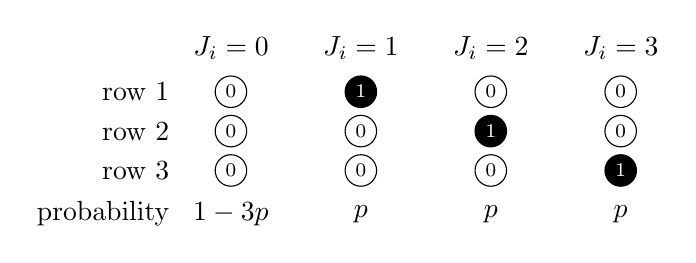
\begin{tikzpicture}[x=1.65cm,y=0.5cm,
  bit/.style={circle,draw,minimum size=4mm,inner sep=0pt},
  present/.style={bit,fill=black,text=white}]
  \foreach \x/\y in {0/1,0/2,0/3,1/1,1/2,2/1,2/3,3/2,3/3}
    \node[bit] at (\x,\y) {\scriptsize 0};
  \foreach \x/\y in {1/3,2/2,3/1}
    \node[present] at (\x,\y) {\scriptsize 1};
  \node at (0,4.1) {$J_i=0$};
  \node at (1,4.1) {$J_i=1$};
  \node at (2,4.1) {$J_i=2$};
  \node at (3,4.1) {$J_i=3$};
  \node at (0,-0.1) {$1-3p$};
  \foreach \x in {1,2,3} {\node at (\x,-0.1) {$p$};}
  \node[anchor=east] at (-0.4,3) {row 1};
  \node[anchor=east] at (-0.4,2) {row 2};
  \node[anchor=east] at (-0.4,1) {row 3};
  \node[anchor=east] at (-0.4,-0.1) {probability};
\end{tikzpicture}
\caption{One coordinate of the sparse coupling, illustrated with three
rows and $3p<1$. Each row contains this coordinate with probability $p$;
the union contains it with probability $3p$. Making these choices
independently across coordinates gives the required product laws.}
\label{fig:coupling}
\end{figure}

\emph{(b) The family of $L$-fold unions.} Define
\[
\mathcal F
=\{D_1\cup\cdots\cup D_L:D_1,\ldots,D_L\in\mathcal D\}.
\]
On the event in~\eqref{eq:all-good}, $R\in\mathcal F$. Since $R$ has law
$\mu_q$,
\[
\mu_q(\mathcal F)=\mathbb P(R\in\mathcal F)
\ge\frac{31}{32}\ge\frac12.
\]

\emph{(c) Same exceptional sets.} A union of $32$ members of $\mathcal F$ is a
union of $32L$ members of $\mathcal D$. Conversely, a union of $32L$ members
of $\mathcal D$ is a union of $32$ members of $\mathcal F$, by grouping the
tuple into $32$ blocks of length $L$. Hence, by
\eqref{eq:exceptional-definition},
\[
E_{32}(\mathcal F)=E_{32L}(\mathcal D)=E_k(\mathcal D).
\]

\emph{(d) Conclusion.} By (b), Proposition~\ref{prop:half-density} applies to
$\mathcal F$ at density $q$ and shows that $E_{32}(\mathcal F)$ is
$(q/L)$-small. By (c) and $q/L=p$, $E_k(\mathcal D)$ is $p$-small.

\step{Case 2: $Lp\ge1$}
Set
\[
t=\frac{p-1/L}{1-1/L}.
\]
Then $t\in[0,1)$, because $1/L\le p<1$. Independently for each coordinate $i$:
choose a \emph{mandatory row} uniformly among the $L$ rows and put $i$ in that
row; conditionally on this choice, put $i$ in each other row independently
with probability $t$. Let $R_j$ be the set of coordinates put in row $j$. For
each fixed $j$,
\[
\mathbb P(i\in R_j)
=\frac1L+\left(1-\frac1L\right)t=\frac1L+\Bigl(p-\frac1L\Bigr)=p,
\]
and the events $\{i\in R_j\}$, $i\in[N]$, are independent because the choices
at different coordinates are independent. So each $R_j$ has law $\mu_p$. In
every outcome each coordinate lies in its mandatory row, so
$R_1\cup\cdots\cup R_L=[N]$.

By~\eqref{eq:all-good} the event that all $L$ rows lie in $\mathcal D$ has
positive probability, so some outcome gives $D_1,\ldots,D_L\in\mathcal D$ with
$D_1\cup\cdots\cup D_L=[N]$. Repeating this tuple $32$ times gives $k=32L$
members of $\mathcal D$ whose union is $[N]$. Every $S\subseteq[N]$ is
contained in this union, so $E_k(\mathcal D)=\varnothing$, which is covered at
cost zero by the empty family. The boundary case $Lp=1$ is included, with
$t=0$.
\end{proof}

\section{Verification checklist}
\label{sec:checklist}

The following steps carry the proof and should be checked first.

\begin{enumerate}
\item \textbf{Residual tuples in Lemma~\ref{lem:covering} (Steps 4, 5, 7).}
The survival probability $(1-\pi)^{m^2}$ requires the $m$ edges of a tuple to
be pairwise distinct. Check that the definition of $\mathcal C_2$ (Step~4),
the covering argument (Step~5) and the probability computation (Step~7) all
refer to distinct tuples, and that over-counting by $W_m$ (Step~6) is
legitimate. The boxed note in Step~4 records how the source's wording was
read.
\item \textbf{Extension bound \eqref{eq:cov-ext} (Lemma~\ref{lem:covering},
Step~2).} Each trace $I=e\cap B$ of a regular edge satisfies $d(I)\le T$, and
there are at most $\sum_{i\le r}\binom{|B|}{i}$ traces. This single bound
gives both the cost of $\mathcal C_1$ (Step~3) and the recursion for $W_\ell$
(Step~6).
\item \textbf{Exponent arithmetic \eqref{eq:cov-arith}
(Lemma~\ref{lem:covering}, Step~8).} With $m=2^{12h}$, $T=2^{4h}$,
$\pi=2^{-8h}$: $4h+13rh+1\le2^{4h}=\pi m$.
\item \textbf{Normalization in Proposition~\ref{prop:half-density}, Step~1(b).}
$\widehat f(U)=(q/(1-q))^{|U|/2}b(U)$, so that
$q^{|U|}w(U)=(1-q)^{|U|}\widehat f(U)^2\le\widehat f(U)^2$.
\item \textbf{Signed identity \eqref{eq:signed-identity}
(Proposition~\ref{prop:half-density}, Step~2).} Check
$\widetilde P(0,\ldots,0)=0$, the termwise vanishing \eqref{eq:signed-zero},
and that the $U$-term of the expansion factors over the $32$ rows as
$\prod_j\kappa_U(x_j)$ with the factor $(1-q)^{32|U|}$ split as $(1-q)^{|U|}$
per row.
\item \textbf{Constants in Proposition~\ref{prop:half-density}, Steps 3--4.}
$70=64+6$ gives $c_\rho(\mathcal G_0)\le2^{-6}$. Occupied bins have $h\ge64r$,
with strictness coming from $U\notin\mathcal G_0$. The lemma's hypothesis
\eqref{eq:bin-hyp} holds. The bin sum $\sum2^{12h}2^{-16h}$ in
\eqref{eq:bin-power} is below $2^{-32}$.
\item \textbf{Couplings (Section~\ref{sec:density}).} In Case~1 each row has
law $\mu_p$ and the union has law $\mu_{Lp}$; $E_{32}(\mathcal
F)=E_{32L}(\mathcal D)$; and $q/L=p$. In Case~2, $t\in[0,1)$, each row has
law $\mu_p$, and the union is $[N]$. In both cases only the union bound
\eqref{eq:all-good} is applied to the dependent rows.
\end{enumerate}

Outside the proof of Theorem~\ref{thm:main}, the proof of
Corollary~\ref{cor:two-union} relies on external statements that we could not
check; see the boxed note there.

\begin{thebibliography}{99}

\bibitem{AscoliEtAl26}
Ruben Ascoli, Xiaoyu He, Jinyoung Park, and Michel Talagrand,
\emph{A reformulation of the discrete Convexity Conjecture via
$k$-thresholds},
arXiv:2608.11183v1, 2026.
\href{https://arxiv.org/abs/2608.11183v1}{arXiv:2608.11183v1}.

\bibitem{EllisFilmusFriedgut12}
David Ellis, Yuval Filmus, and Ehud Friedgut,
\emph{Triangle-intersecting families of graphs},
Journal of the European Mathematical Society \textbf{14} (2012),
no.~3, 841--885.
\href{https://doi.org/10.4171/JEMS/320}{doi:10.4171/JEMS/320}.

\bibitem{FischerPerson25}
Thomas Fischer and Yury Person,
\emph{Further remarks on fractional vs. expectation thresholds},
arXiv:2505.21782v1, 2025.
\href{https://doi.org/10.48550/arXiv.2505.21782}{doi:10.48550/arXiv.2505.21782}.

\bibitem{Friedgut08}
Ehud Friedgut,
\emph{On the measure of intersecting families, uniqueness and stability},
Combinatorica \textbf{28} (2008), no.~5, 503--528.
\href{https://doi.org/10.1007/s00493-008-2318-9}{doi:10.1007/s00493-008-2318-9}.

\bibitem{HuaSongTudose26}
Dongming (Merrick) Hua, Antoine Song, and Stefan Tudose,
\emph{On Talagrand's Convexity Conjecture},
arXiv:2605.10908v2, 2026.
\href{https://arxiv.org/abs/2605.10908v2}{arXiv:2605.10908v2}.

\bibitem{Li26}
Chen Li,
\emph{On $p$-spread measures},
arXiv:2609.08967v1, 2026.
\href{https://arxiv.org/abs/2609.08967v1}{arXiv:2609.08967v1}.

\bibitem{ODonnell14}
Ryan O'Donnell,
\emph{Analysis of Boolean Functions},
Cambridge University Press, Cambridge, 2014.
Author's corrected text, 2021:
\href{https://arxiv.org/abs/2105.10386v1}{arXiv:2105.10386v1}.

\bibitem{OpenAIThreshold26}
OpenAI,
\emph{Integral and fractional expectation thresholds are equivalent},
OpenAI Math Release preprint
\href{https://github.com/openai/math/blob/main/preprints/Integral-and-fractional-expectation-thresholds-are-equivalent-September-23-2026/paper.pdf}{OAI:Integral-and-fractional-expectation-thresholds-are-equivalent-September-23-2026},
2026.

\bibitem{Park26}
Jinyoung Park,
\emph{A dimension-free comparison between expectation thresholds and
fractional expectation thresholds},
arXiv:2609.14681v1, 2026.
\href{https://arxiv.org/abs/2609.14681v1}{arXiv:2609.14681v1}.

\bibitem{ParkPham24}
Jinyoung Park and Huy Tuan Pham,
\emph{On a conjecture of Talagrand on selector processes and a consequence
on positive empirical processes},
Annals of Mathematics \textbf{199} (2024), no.~3, 1293--1321.
\href{https://doi.org/10.4007/annals.2024.199.3.6}{doi:10.4007/annals.2024.199.3.6}.

\bibitem{Talagrand10}
Michel Talagrand,
\emph{Are many small sets explicitly small?},
Proceedings of the Forty-Second ACM Symposium on Theory of Computing,
ACM, New York, 2010, 13--36.
\href{https://doi.org/10.1145/1806689.1806693}{doi:10.1145/1806689.1806693}.

\bibitem{Talagrand21}
Michel Talagrand,
\emph{Upper and Lower Bounds for Stochastic Processes:
Decomposition Theorems},
2nd ed., Ergebnisse der Mathematik und ihrer Grenzgebiete, 3.~Folge,
vol.~60, Springer, Cham, 2021.
\href{https://doi.org/10.1007/978-3-030-82595-9}{doi:10.1007/978-3-030-82595-9}.

\end{thebibliography}

\end{document}
